\documentclass{beamer}
\usepackage{graphicx}
\usepackage{amsmath}

\title{Detailed Explanations of Monetary Policy Concepts}
\author{Charles Ancel}
\date{July 15, 2024}

\begin{document}

\begin{frame}
    \titlepage{}
\end{frame}

\section{Introduction}
\begin{frame}
    \frametitle{Introduction}
    My name is Charles Ancel, my UIN is 654604114, and this is my ID\@. I'm currently enrolled in ECON 425 during the Summer Session. This assignment is part of the requirement from the University regarding the College of LAS's identity verification policy for LAS Online-certified classes. For the answers in this assignment, I did not use any form of Artificial Intelligence (AI) help, such as Chat-GPT or similar, and thus my answers will accurately and fairly reflect my own learning from this course.
\end{frame}

\section{Federal Reserve's Process for Implementing Monetary Policy}
\begin{frame}
    \frametitle{Federal Reserve's Process for Implementing Monetary Policy}
    \textbf{Question 1:} Explain the actual process the Federal Reserve takes to implement monetary policy. In particular:
    \begin{itemize}
        \item What is the main instrument of the Fed's monetary policy and is it in its direct control?
        \item How is monetary policy decided in the FOMC meetings?
        \item How is the monetary policy decision announced to the public?
        \item How is the FOMC decision of monetary policy implemented by the New York Fed's Open Market Trading Desk?
    \end{itemize}
\end{frame}

\begin{frame}
    \frametitle{Main Instrument of the Fed's Monetary Policy}
    \textbf{1.1 Main Instrument of the Fed's Monetary Policy:} The main instrument of the Fed's monetary policy is the federal funds rate, which is the interest rate at which banks lend reserves to each other overnight. This rate is influenced through open market operations but is not directly controlled by the Fed.
\end{frame}

\begin{frame}
    \frametitle{Decision Process in FOMC Meetings}
    \textbf{1.2 Decision Process in FOMC Meetings:} Monetary policy is decided in the Federal Open Market Committee (FOMC) meetings, where members review economic data, consider forecasts, and discuss economic conditions before voting on the appropriate level for the federal funds rate. The FOMC meets eight times a year, but can meet more often if needed.
\end{frame}

\begin{frame}
    \frametitle{Public Announcement}
    \textbf{1.3 Public Announcement:} The monetary policy decision is announced to the public via press releases and statements from the Fed, providing transparency and managing market expectations. The Fed Chair holds a press conference to explain the rationale behind the decision and to answer questions from the media.
\end{frame}

\begin{frame}
    \frametitle{Implementation by the New York Fed}
    \textbf{1.4 Implementation by the New York Fed's Open Market Trading Desk:} The New York Fed's Open Market Trading Desk implements the FOMC's decision by conducting open market operations. This involves buying or selling government securities to influence the supply of reserves in the banking system, which in turn affects the federal funds rate.
\end{frame}

\section{Objectives of Monetary Policy}
\begin{frame}
    \frametitle{Objectives of Monetary Policy}
    \textbf{Question 2:} What are the (main) objectives of monetary policy?
    \begin{itemize}
        \item \textbf{2.1 Price Stability:} One of the main objectives of monetary policy is to maintain price stability, which means keeping inflation low and stable. This helps maintain the purchasing power of money and fosters economic growth.
        \item \textbf{2.2 Full Employment:} Another objective is to achieve full employment, where all who are willing and able to work can find employment. This ensures that resources are fully utilized and helps improve living standards.
    \end{itemize}
\end{frame}

\begin{frame}
    \frametitle{Central Bank's Loss Function}
    \textbf{2.3 Loss Function:} The central bank's loss function reflects the trade-offs between these objectives. It typically includes terms for both inflation and output variability:
    \begin{equation*}
        L = \lambda {(\pi_t - \pi^*)}^2 + {(y_t - y^*)}^2
    \end{equation*}
    where \(\pi_t\) is the inflation rate, \(\pi^*\) is the target inflation rate, \(y_t\) is the output, and \(y^*\) is the potential output. The loss function shows how deviations from the targets for inflation and output are weighted and minimized.
\end{frame}

\section{Term Structure of Interest Rates}
\begin{frame}
    \frametitle{Term Structure of Interest Rates}
    \textbf{Question 3:} Explain what is the term structure of interest rates and how this relates to the objectives of monetary policy.
    \begin{itemize}
        \item \textbf{3.1 Concept of Term Structure:} The term structure of interest rates, or yield curve, represents the relationship between interest rates of bonds with different maturities. Typically, longer-term bonds have higher interest rates than shorter-term bonds due to the higher risk and time involved.
        \item \textbf{3.2 Relevance to Monetary Policy:} Monetary policy influences the term structure by setting short-term interest rates, which affect longer-term rates. For example, when the Fed raises the federal funds rate, short-term interest rates increase, which can lead to higher long-term rates. This helps the Fed achieve its objectives of price stability and full employment by influencing borrowing costs, consumer spending, and investment decisions.
    \end{itemize}
\end{frame}

\begin{frame}
    \frametitle{Graph: Term Structure of Interest Rates}
    \begin{center}
        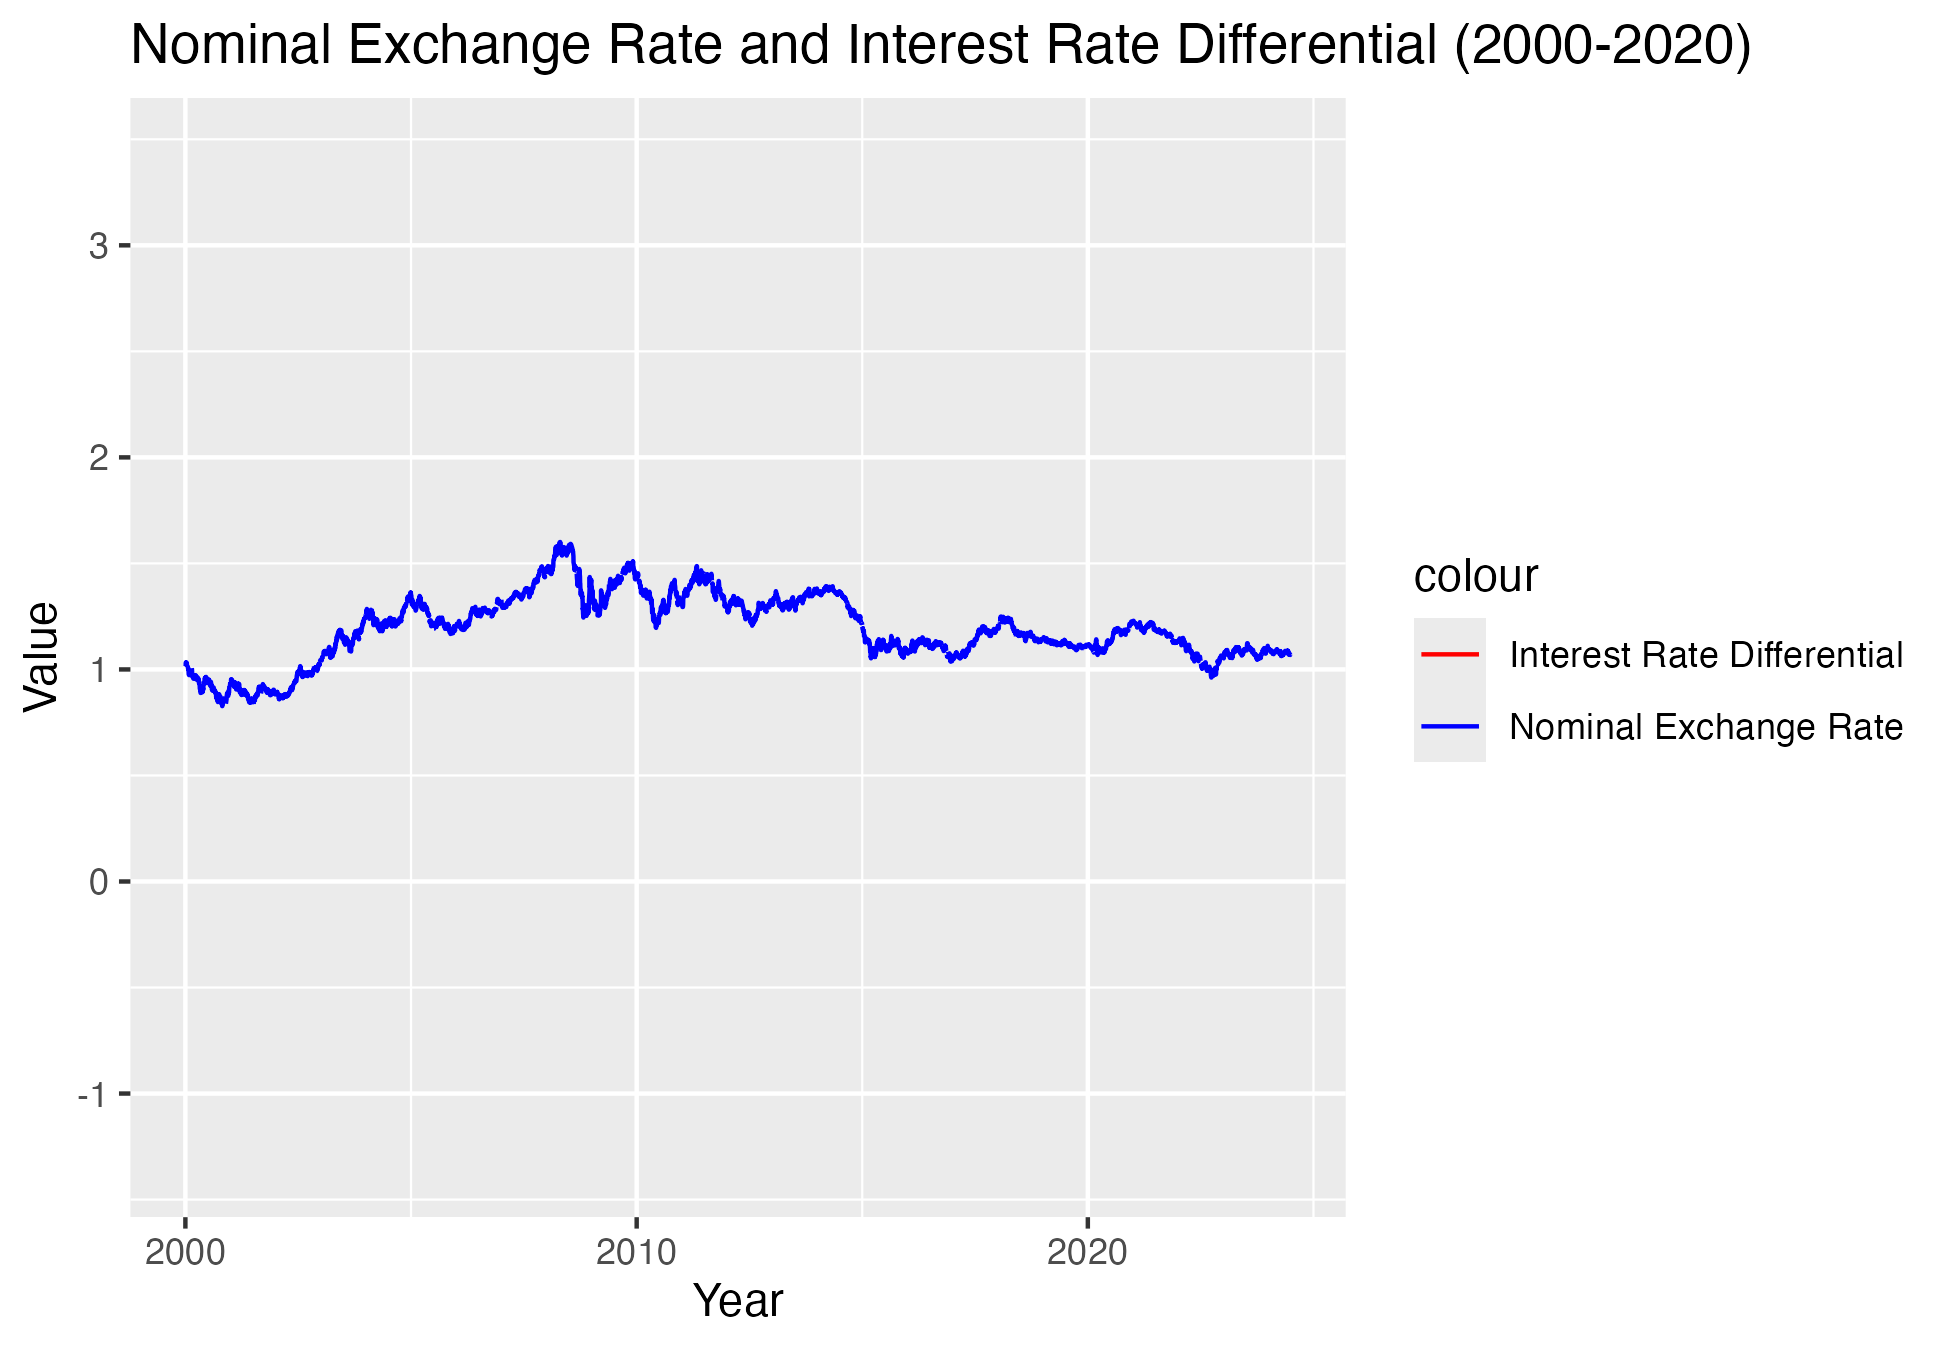
\includegraphics[width=0.9\textwidth]{/Users/cancel/Personal/Coursework/Econ425/VA2/R/Nominal_Exchange_Rate_and_Interest_Rate_Differential.png}
    \end{center}
    \textbf{Explanation:} This graph shows the relationship between the nominal exchange rate (in blue) and the interest rate differential (in red) over the period from 2000 to 2020. The nominal exchange rate is influenced by the difference between domestic and foreign interest rates. When the interest rate differential increases, the nominal exchange rate typically appreciates.
\end{frame}

\begin{frame}
    \frametitle{Graph: Term Structure of Interest Rate Explained}

    \textbf{Explanation:} This graph shows the relationship between the nominal exchange rate (in blue) and the interest rate differential (in red) over the period from 2000 to 2020. The nominal exchange rate is influenced by the difference between domestic and foreign interest rates. When the interest rate differential increases, the nominal exchange rate typically appreciates.
    

\end{frame}

\section{MP Curve and Optimal Monetary Policy}
\begin{frame}
    \frametitle{MP Curve and Optimal Monetary Policy}
    \textbf{Question 4:} Explain when does the MP curve (of chapter 2) actually represent optimal monetary policy and when it doesn’t.
    \begin{itemize}
        \item \textbf{4.1 Optimal Policy Representation:} The MP curve shows the relationship between the real interest rate and inflation. It represents optimal policy when it aligns with the central bank's objectives of price stability and full employment. This means the central bank adjusts the real interest rate in response to changes in inflation to maintain economic stability.
        \item \textbf{4.2 Non-Optimal Conditions:} The MP curve may not be optimal if it doesn't account for other economic conditions or shocks, such as supply-side disturbances or financial market instability. In such cases, following the MP curve strictly could lead to excessive inflation volatility or failing to address output gaps effectively, which could harm the economy.
    \end{itemize}
\end{frame}

\begin{frame}
    \frametitle{Graph: MP Curve}
    \begin{center}
        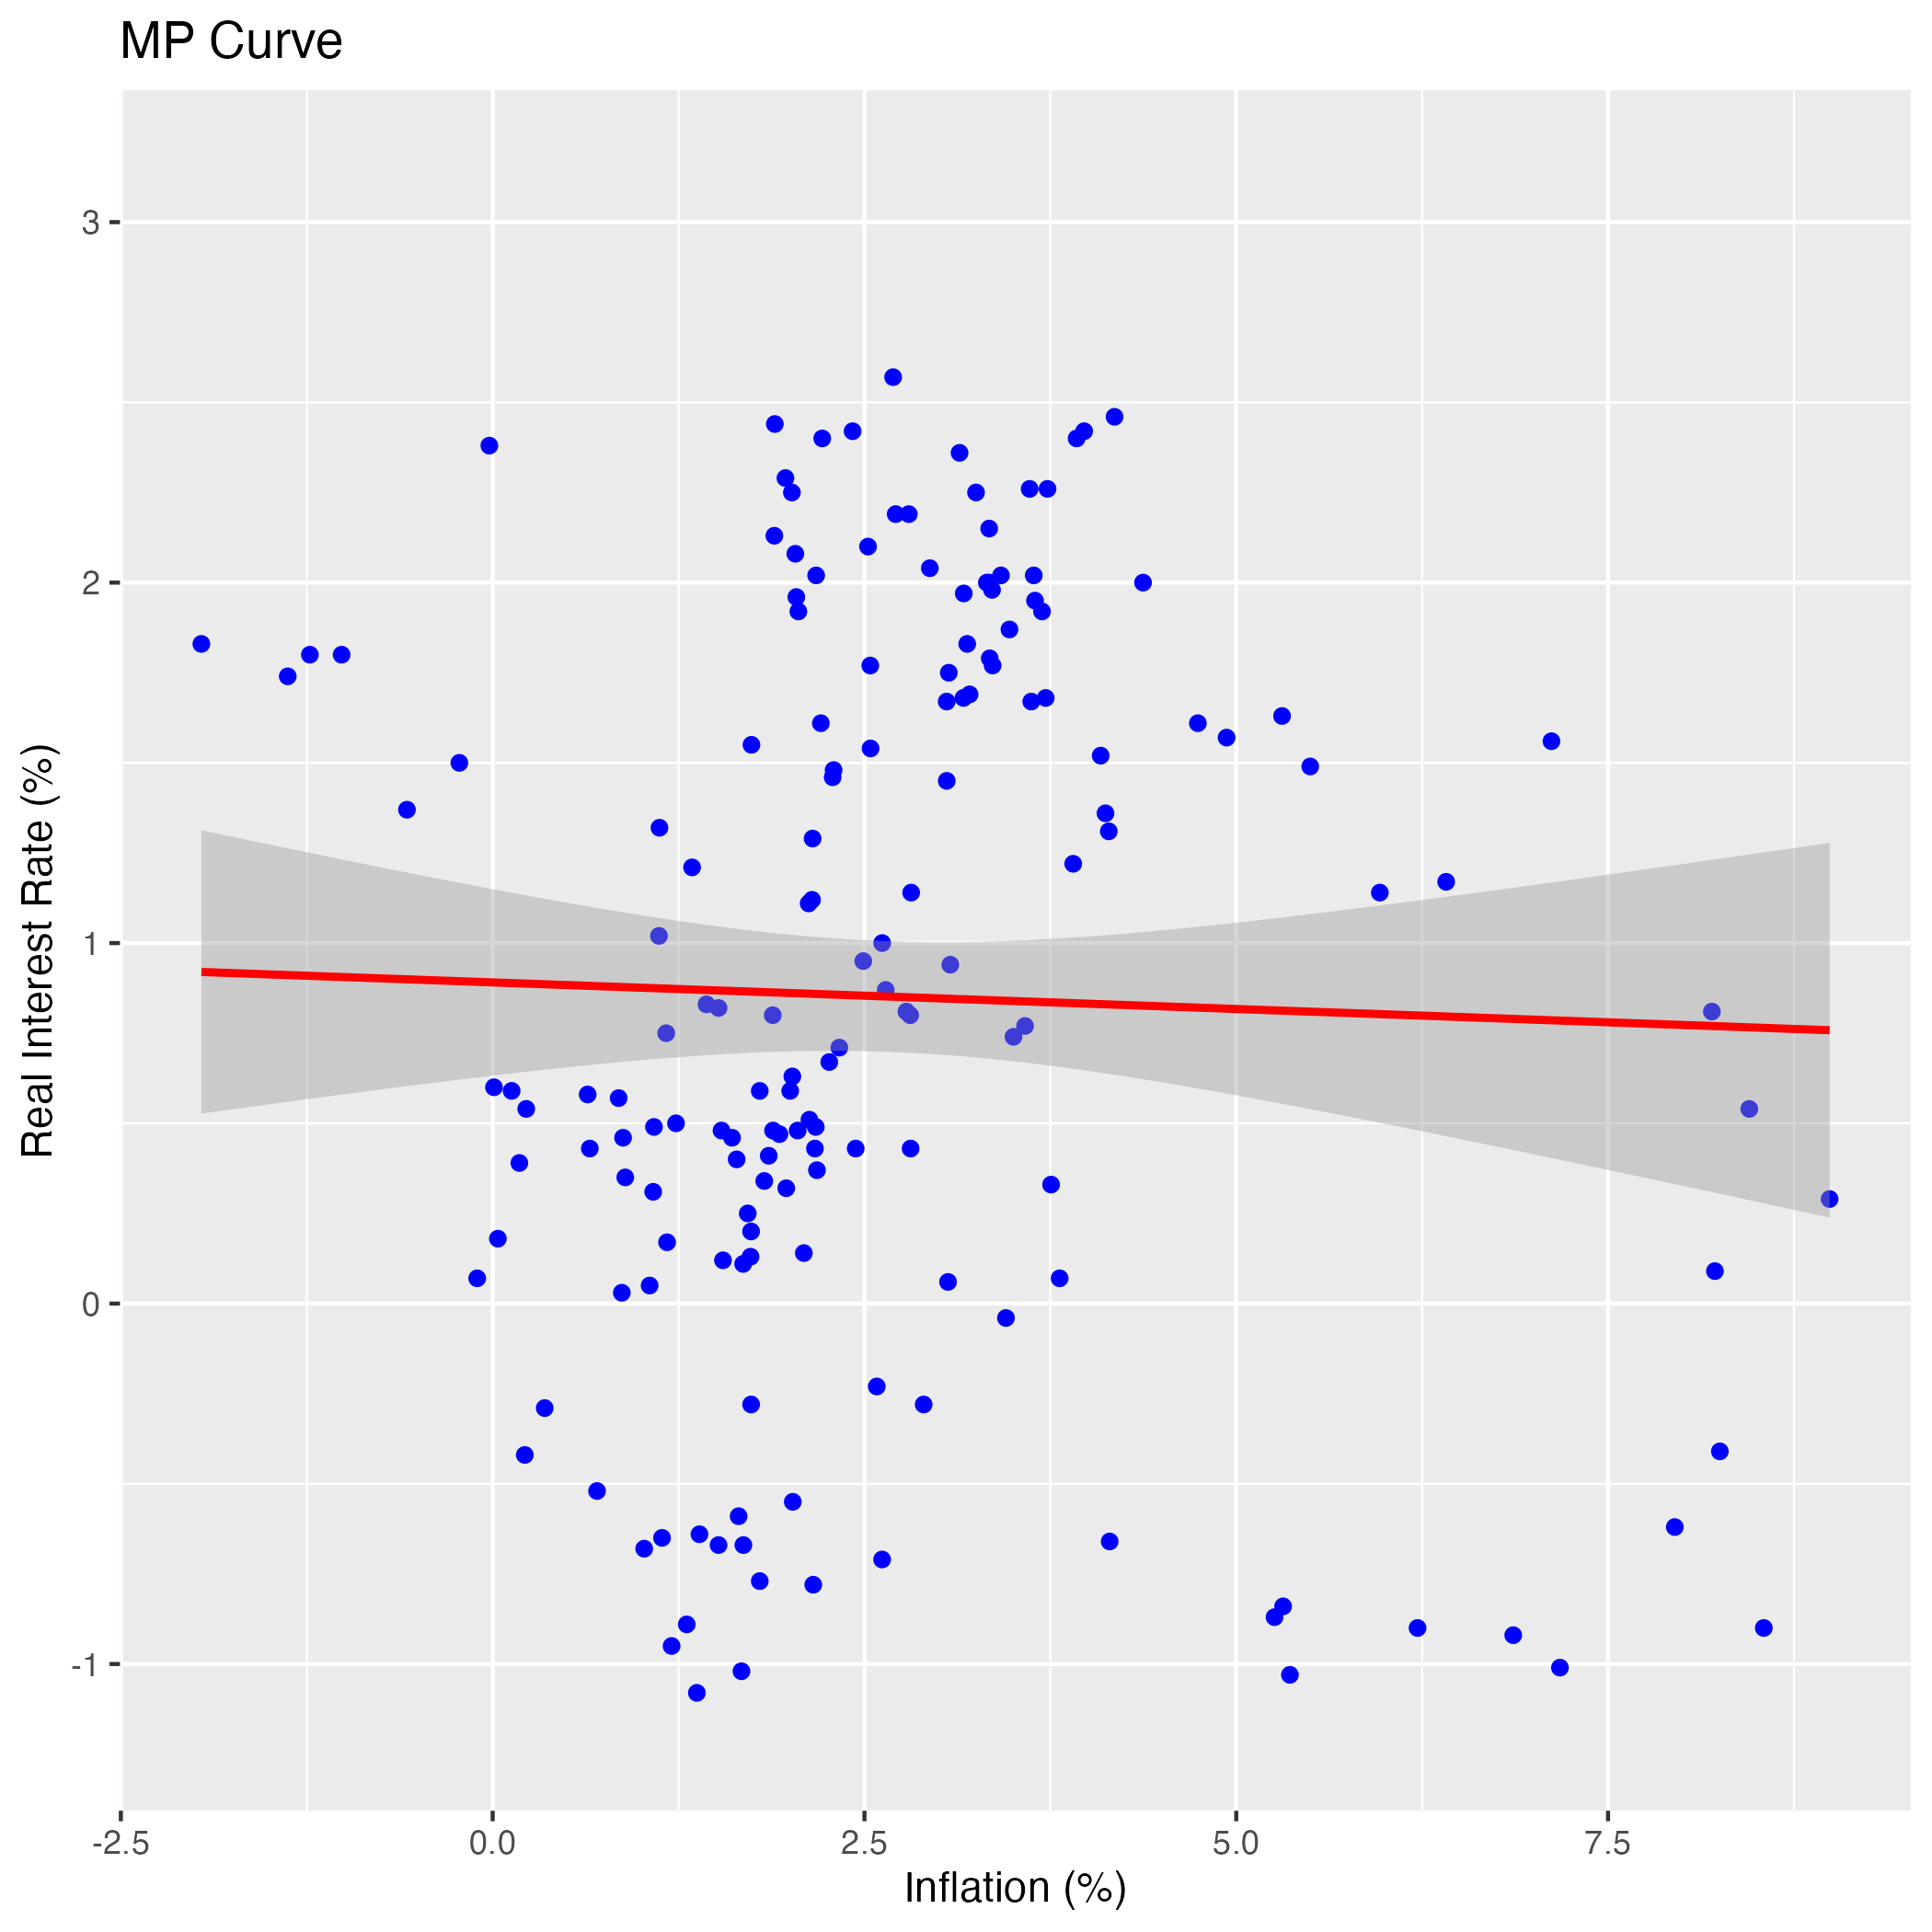
\includegraphics[width=0.8\textwidth]{/Users/cancel/Personal/Coursework/Econ425/VA2/R/MP_Curve.png}
    \end{center}
    \textbf{Explanation:} This graph represents the MP curve, showing the relationship between the real interest rate and inflation. A negative slope indicates that higher inflation leads to a lower real interest rate set by the central bank. This curve is used to illustrate how monetary policy can stabilize the economy by adjusting interest rates in response to inflation changes.
\end{frame}

\begin{frame}
    \frametitle{Graph: MP Curve Explained}
\textbf{Explanation:} This graph represents the MP curve, showing the relationship between the real interest rate and inflation. A negative slope indicates that higher inflation leads to a lower real interest rate set by the central bank. This curve is used to illustrate how monetary policy can stabilize the economy by adjusting interest rates in response to inflation changes.
\end{frame}
    
\section{The Taylor Rule}
\begin{frame}
    \frametitle{The Taylor Rule}
    \textbf{Question 5:} Is the Taylor Rule optimal policy? If yes, why? If not, then why is it helpful?
    \begin{itemize}
        \item \textbf{5.1 Definition and Formula:} The Taylor Rule provides a guideline for setting interest rates based on inflation and output gaps:
        \begin{equation*}
            i_t = r^* + \pi_t + 0.5(\pi_t - \pi^*) + 0.5(y_t - y^*)
        \end{equation*}
        where \(i_t\) is the nominal interest rate, \(r^*\) is the real equilibrium interest rate, \(\pi_t\) is the inflation rate, \(\pi^*\) is the target inflation rate, \(y_t\) is the output, and \(y^*\) is the potential output.
        \item \textbf{5.2 Optimality and Usefulness:} While not always optimal, the Taylor Rule is useful for its simplicity and transparency. It helps guide expectations and improve policy credibility by providing a clear and predictable framework for setting interest rates. However, it may not always be optimal because it doesn't account for all possible economic conditions and shocks. In some situations, more flexibility in policy-making might be needed.
    \end{itemize}
\end{frame}

\section{Dangers of Not Following the Taylor Principle}
\begin{frame}
    \frametitle{Dangers of Not Following the Taylor Principle}
    \textbf{Question 6:} What are the dangers of failing to follow the Taylor principle when facing high inflation?
    \begin{itemize}
        \item \textbf{6.1 Taylor Principle Explanation:} The Taylor Principle states that the central bank should raise nominal interest rates by more than the increase in inflation to stabilize the economy. This means if inflation rises by 1%, the nominal interest rate should rise by more than 1% to prevent inflation from spiraling out of control.
        \item \textbf{6.2 Consequences of Ignoring the Principle:} Failing to follow the Taylor Principle during high inflation can lead to runaway inflation. If the central bank does not raise interest rates sufficiently, real interest rates (nominal rates adjusted for inflation) fall, which boosts aggregate demand and further increases inflation. This can result in an inflationary spiral, where prices keep rising uncontrollably, eroding purchasing power and economic stability.
    \end{itemize}
\end{frame}

\begin{frame}
    \frametitle{Graph: Taylor Principle}
    \begin{center}
        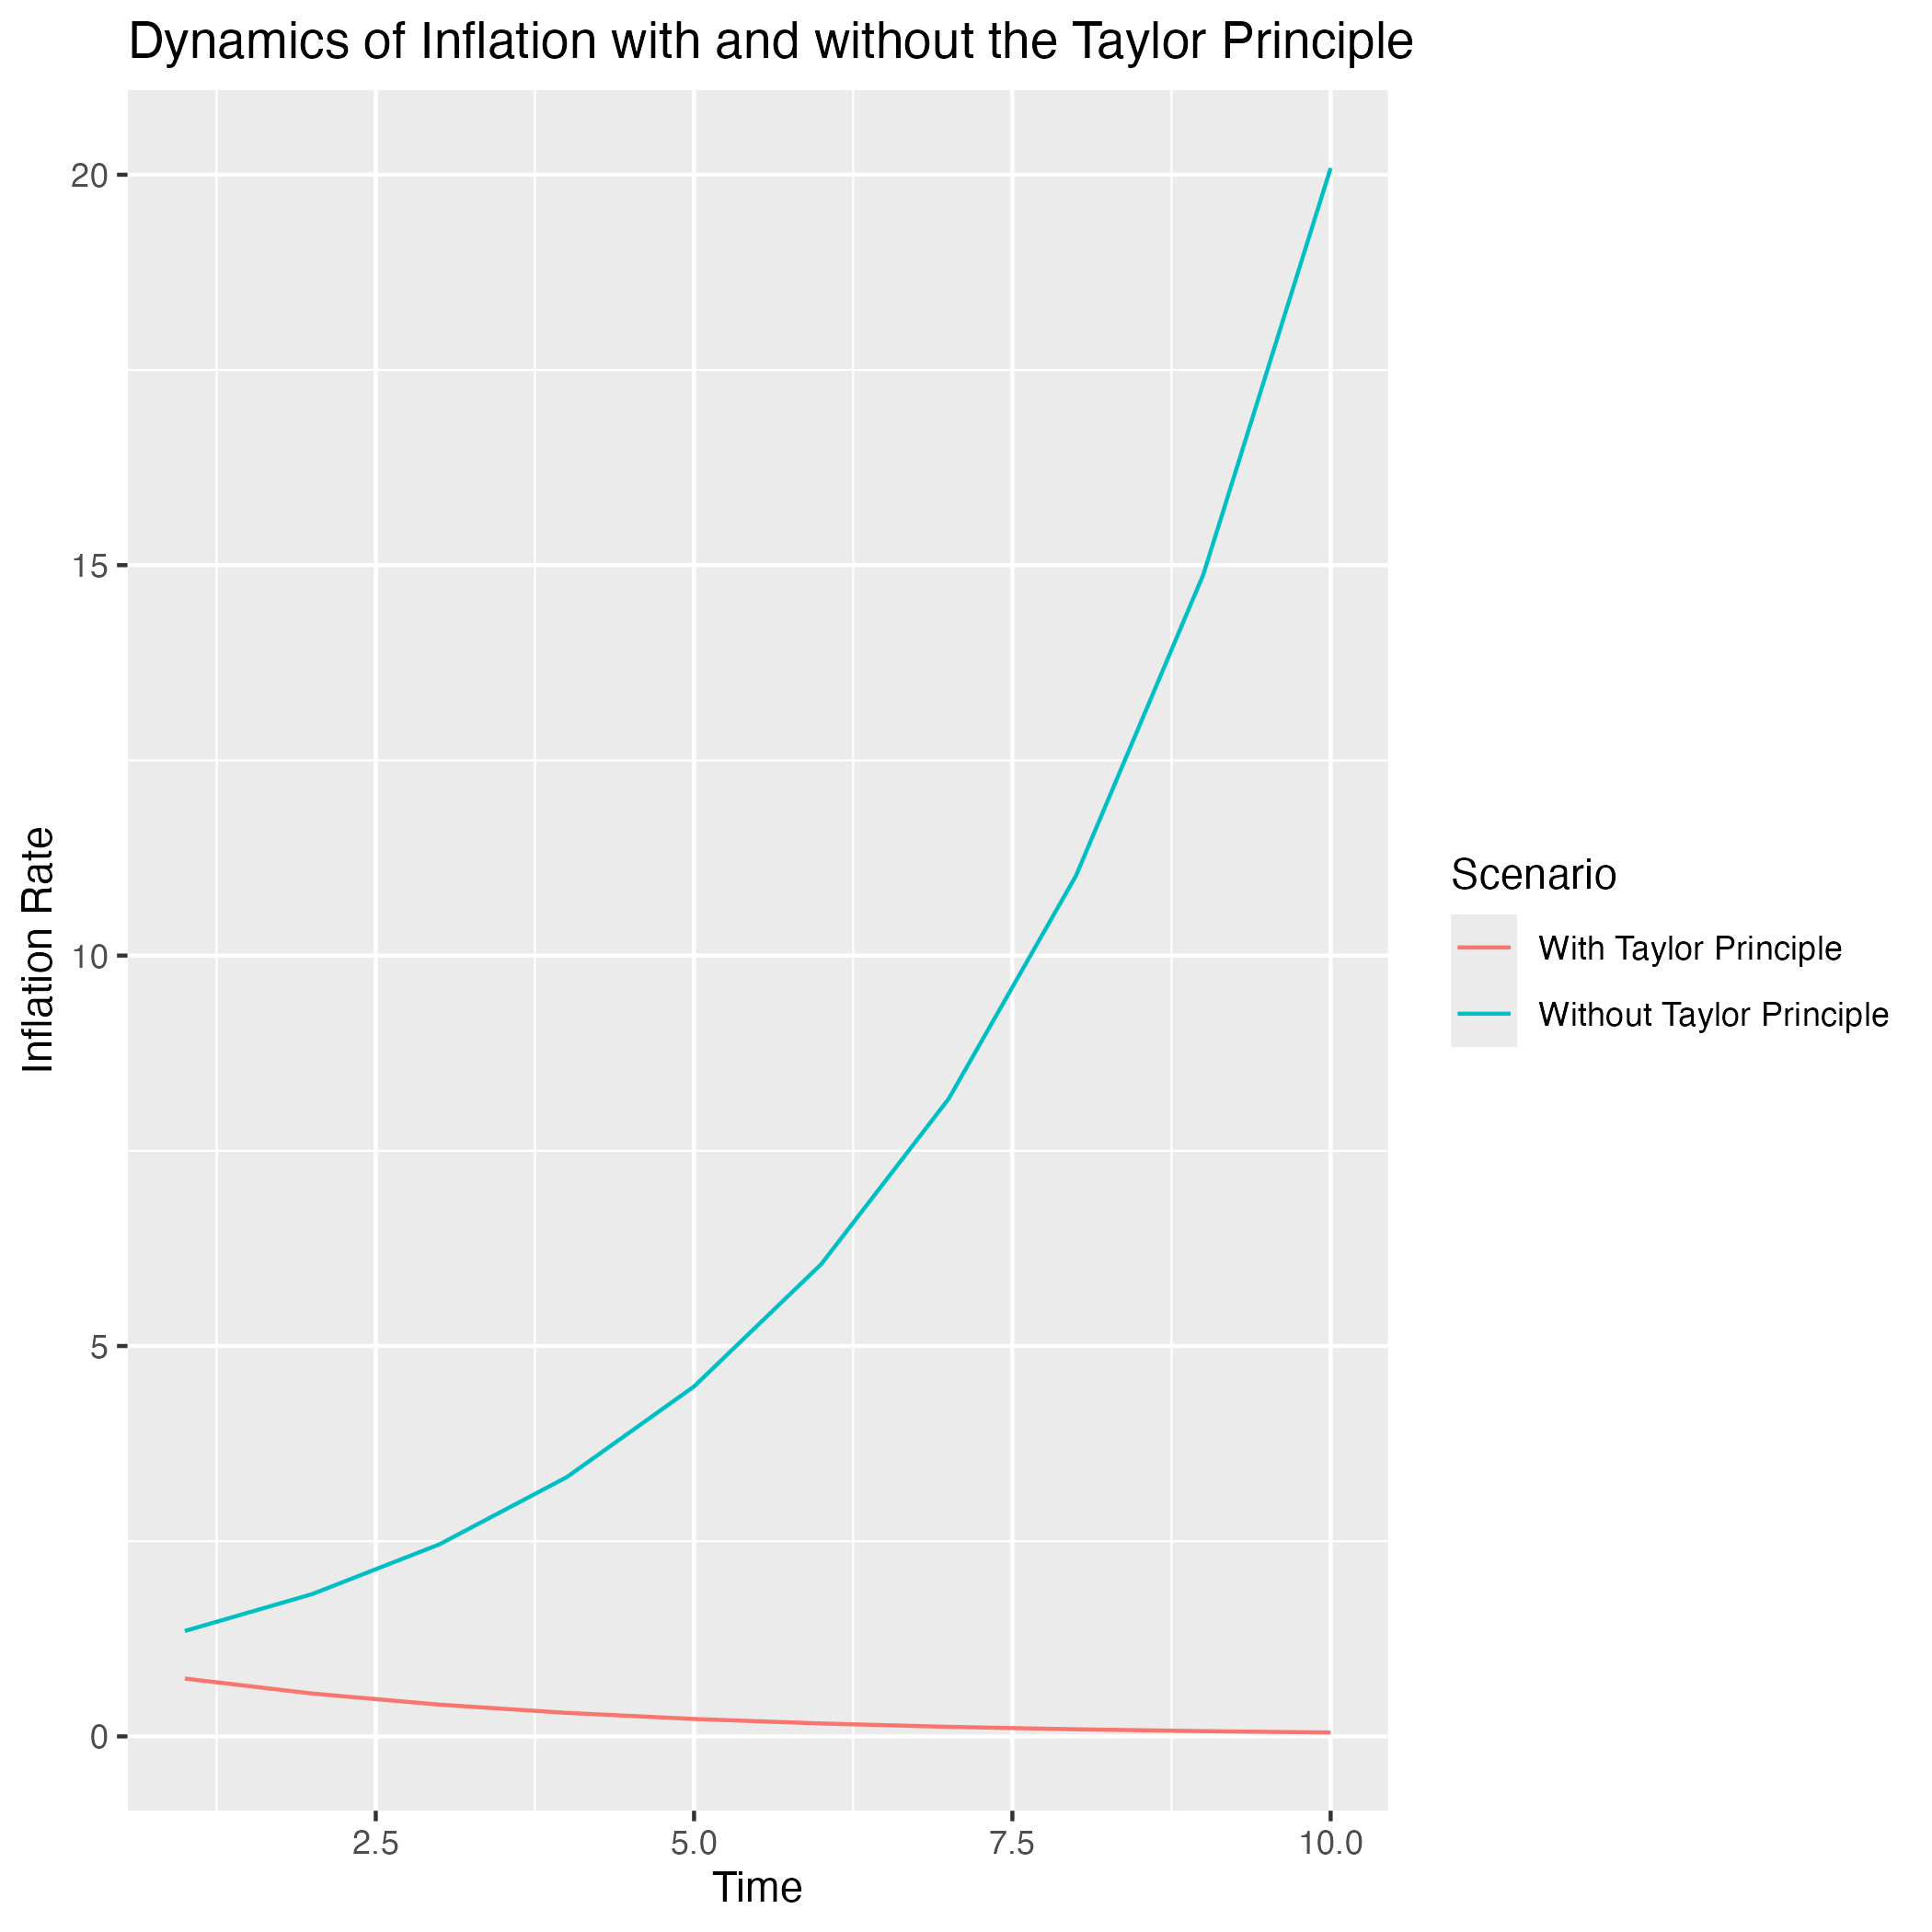
\includegraphics[width=0.8\textwidth]{/Users/cancel/Personal/Coursework/Econ425/VA2/R/InflationDynamics.png}
    \end{center}
    \textbf{Explanation:} This graph illustrates the dynamics of inflation with and without following the Taylor Principle. The red line shows the scenario where the Taylor Principle is followed, resulting in controlled inflation. The blue line represents the scenario without the Taylor Principle, where inflation rises exponentially over time. This demonstrates the importance of adhering to the Taylor Principle to prevent runaway inflation.
\end{frame}

\begin{frame}
    \frametitle{Graph: Taylor Principle Explained}
    \textbf{Explanation:} This graph illustrates the dynamics of inflation with and without following the Taylor Principle. The red line shows the scenario where the Taylor Principle is followed, resulting in controlled inflation. The blue line represents the scenario without the Taylor Principle, where inflation rises exponentially over time. This demonstrates the importance of adhering to the Taylor Principle to prevent runaway inflation.

    

\end{frame}
\section{Optimal Stabilization vs. Optimal Disinflation}
\begin{frame}
    \frametitle{Optimal Stabilization vs. Optimal Disinflation}
    \textbf{Question 7:} What's the difference between optimal stabilization and optimal disinflation? Explain in detail.
    \begin{itemize}
        \item \textbf{7.1 Optimal Stabilization:} Optimal stabilization aims to minimize the variance of both inflation and output by responding to economic shocks in a balanced manner. This involves adjusting monetary policy to smooth out fluctuations in the economy, keeping both inflation and unemployment low and stable.
        \item \textbf{7.2 Optimal Disinflation:} Optimal disinflation focuses on reducing inflation to a lower target level with minimal output loss. This involves a gradual approach to reducing inflation to avoid causing sharp recessions. Disinflation policies need to be carefully managed to ensure that lowering inflation does not lead to a significant increase in unemployment or a severe economic downturn.
    \end{itemize}
\end{frame}

\section{Importance of Expectations in Macroeconomics}
\begin{frame}
    \frametitle{Importance of Expectations in Macroeconomics}
    \textbf{Question 8:} Explain the importance of expectations in macroeconomics. Why do most standard models assume that agents have rational expectations?
    \begin{itemize}
        \item \textbf{8.1 Role of Expectations:} Expectations about future economic conditions influence current behavior. For example, if people expect higher inflation, they may spend more now, increasing current inflation. Expectations affect decisions on spending, saving, and investing, which in turn influence economic outcomes.
        \item \textbf{8.2 Rational Expectations:} Standard models assume rational expectations, meaning people use all available information to make forecasts, leading to more accurate predictions and efficient markets. Rational expectations ensure that economic agents do not systematically make errors in their predictions, which helps stabilize the economy and makes monetary policy more effective.
    \end{itemize}
\end{frame}

\section{The Lucas Critique}
\begin{frame}
    \frametitle{The Lucas Critique}
    \textbf{Question 9:} Explain what is the ``Lucas critique'' and its importance for policy making.
    \begin{itemize}
        \item \textbf{9.1 Explanation of Lucas Critique:} The Lucas Critique argues that traditional econometric models fail to account for changes in policy regimes because they don't consider how agents' behavior changes in response to new policies. If a policy change is anticipated, agents will alter their behavior, making past data unreliable for predicting future outcomes.
        \item \textbf{9.2 Importance for Policy Making:} This critique highlights the need for models that incorporate rational expectations and the impact of policy changes on behavior. It emphasizes the importance of considering how policy shifts will affect expectations and actions of economic agents, making policy analysis more robust and realistic.
    \end{itemize}
\end{frame}

\section{Central Bank Preferences and Policy}
\begin{frame}
    \frametitle{Central Bank Preferences and Policy}
    \textbf{Question 10:} What are the dangers of having a central bank that aligns perfectly with the preferences of the people? What is a possible solution and why?
    \begin{itemize}
        \item \textbf{10.1 Dangers of Alignment:} A central bank too aligned with public preferences may prioritize short-term gains over long-term stability, leading to inflationary policies and economic instability. For example, there might be pressure to keep interest rates low to boost employment in the short term, even if this risks higher inflation in the future.
        \item \textbf{10.2 Solution: Central Bank Independence:} Appointing a conservative central banker who prioritizes inflation control over output stabilization can help mitigate this risk. Central bank independence ensures that monetary policy decisions are made based on long-term economic goals rather than short-term political pressures, balancing long-term stability with short-term flexibility.
    \end{itemize}
\end{frame}

\section{Conclusion}
\begin{frame}
    \frametitle{Conclusion}
    Thank you for your attention. This concludes my discussion on monetary policy concepts. I hope this has provided a clear and comprehensive understanding of the topics. If you have any questions, please feel free to ask.
\end{frame}

\end{document}
